%Suggested order of slides
% slides-nonlinsvm-featuregen
% slides-nonlinsvm-kernel-trick
% slides-nonlinsvm-kernel-poly
% slides-nonlinsvm-rkhs-repr
% slides-nonlinsvm-kernel-rbf
% slides-nonlinsvm-modelsel
% slides-nonlinsvm-uniapprox


\subsection{Feature Generation for Nonlinear Separation}
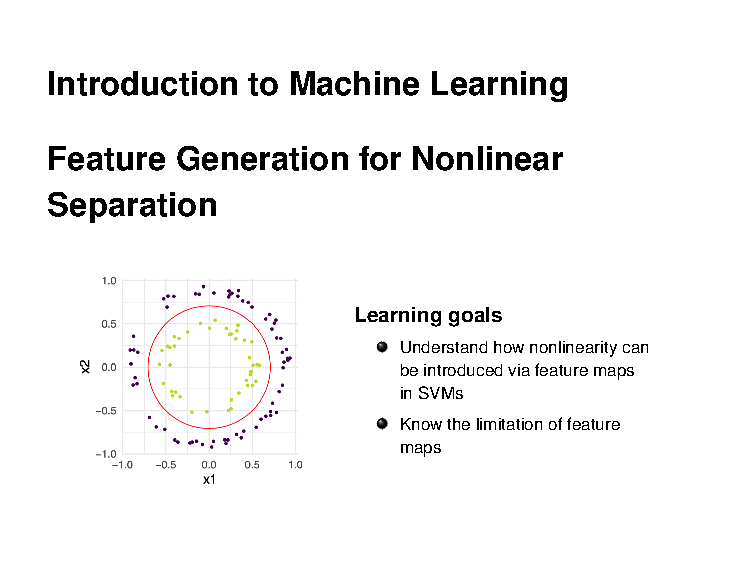
\includepdf[pages=-]{../../slides-pdf/slides-nonlinsvm-featuregen.pdf}

\subsection{The Kernel Trick}
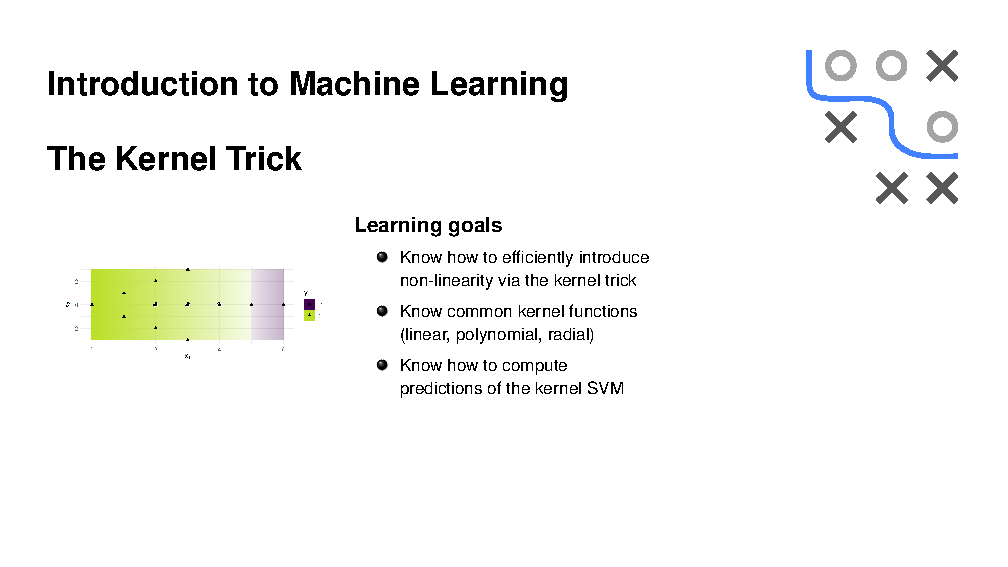
\includepdf[pages=-]{../../slides-pdf/slides-nonlinsvm-kernel-trick.pdf}

\subsection{The Polynomial Kernel}
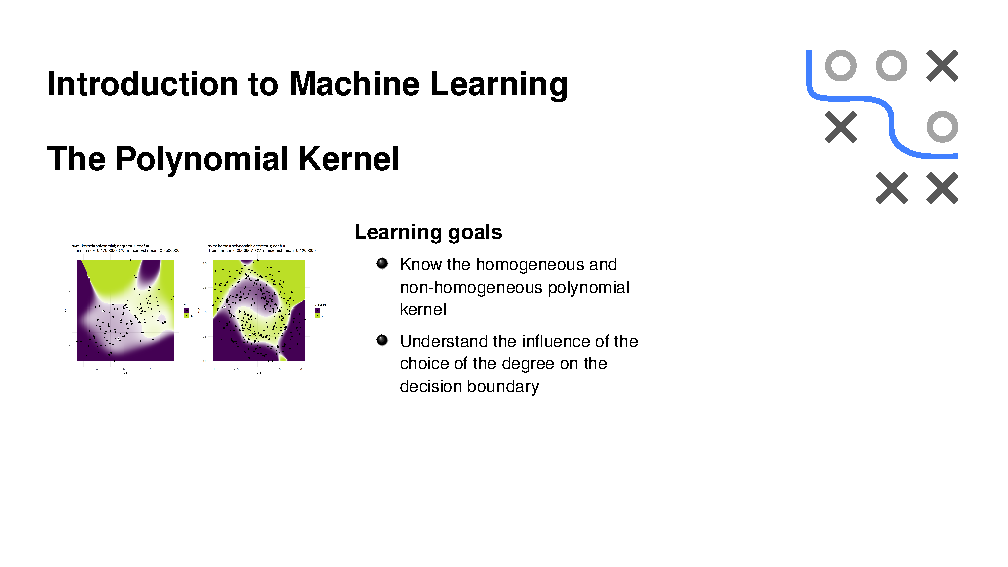
\includepdf[pages=-]{../../slides-pdf/slides-nonlinsvm-kernel-poly.pdf}

\subsection{Reproducing Kernel Hilbert Space and Representer Theorem}
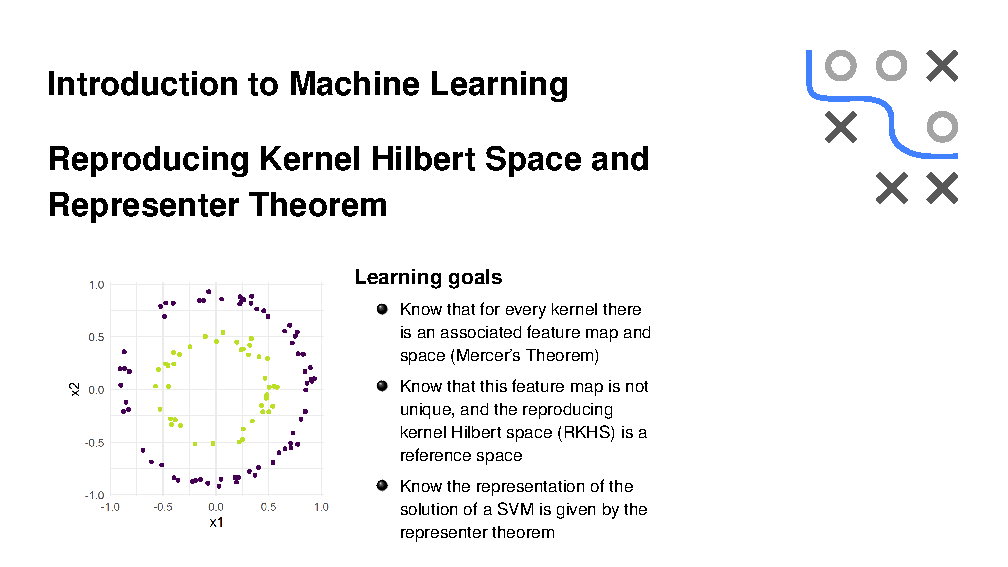
\includepdf[pages=-]{../../slides-pdf/slides-nonlinsvm-rkhs-repr.pdf}

\subsection{The Gaussian RBF Kernel}
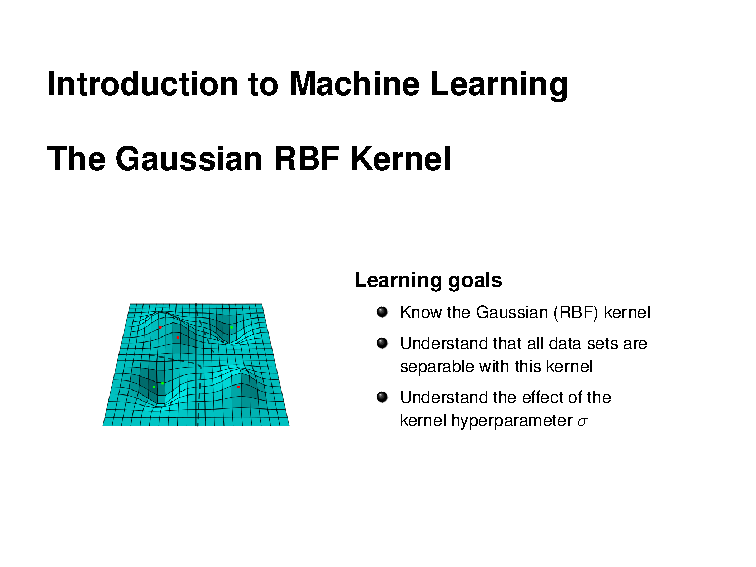
\includepdf[pages=-]{../../slides-pdf/slides-nonlinsvm-kernel-rbf.pdf}

\subsection{SVM Model Selection}
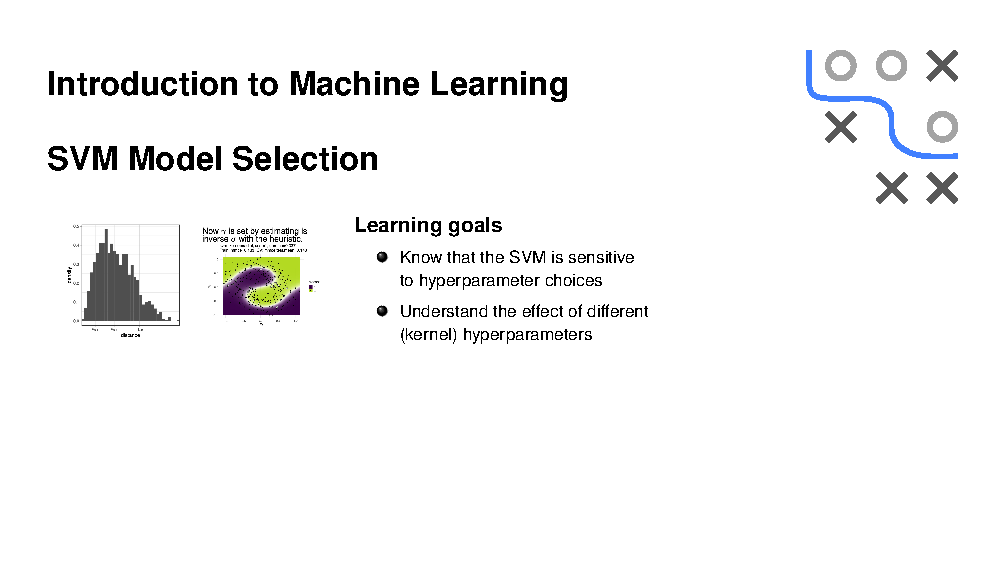
\includepdf[pages=-]{../../slides-pdf/slides-nonlinsvm-modelsel.pdf}

\subsection{Details on Support Vector Machines}
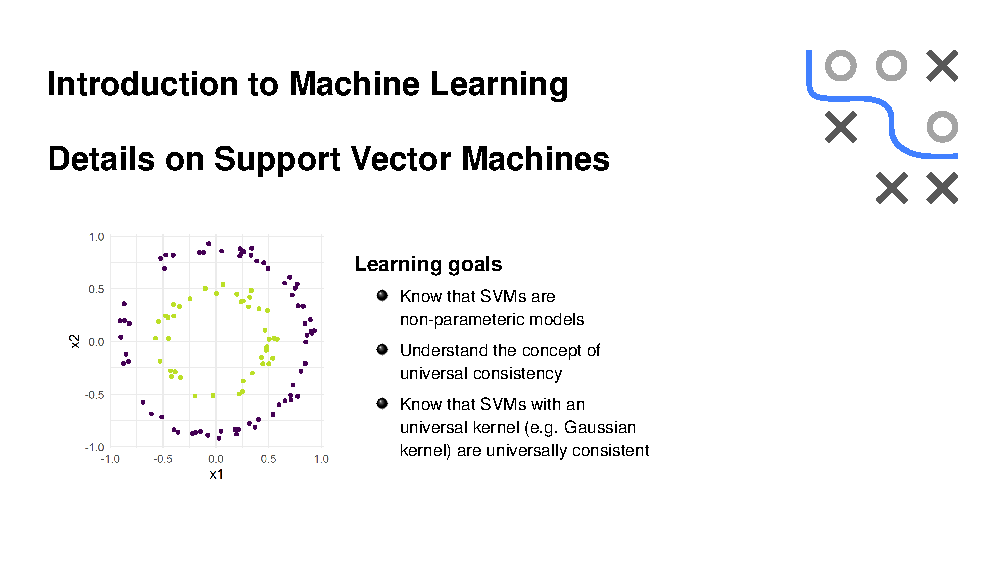
\includepdf[pages=-]{../../slides-pdf/slides-nonlinsvm-uniapprox.pdf}



